\documentclass[tikz,border=8pt]{standalone}
% Shared look for every TikZ diagram. Load with \input{../../tools/tikz-style.tex}
\usepackage[T1]{fontenc}
\usepackage{lmodern}
\renewcommand{\sfdefault}{lmr}  % diagrams use the same serif as the text
\usetikzlibrary{arrows.meta, positioning, shapes.geometric, calc, fit, backgrounds}
\definecolor{cblue}{HTML}{4C78A8}
\definecolor{corange}{HTML}{F58518}
\definecolor{cgreen}{HTML}{54A24B}
\definecolor{cred}{HTML}{E45756}
\definecolor{cpurple}{HTML}{B279A2}
\definecolor{cgrey}{HTML}{6B6B6B}
\tikzset{
  every picture/.style={font=\sffamily, line width=1.2pt},
  box/.style={draw=#1, fill=#1!12, rounded corners=4pt, align=center, inner sep=7pt, minimum height=1.1cm},
  box/.default=cgrey,
  arrow/.style={-{Stealth[length=3mm]}, draw=cgrey, line width=1.4pt},
  title/.style={font=\sffamily\bfseries\Large},
  note/.style={font=\sffamily\small, text=cgrey, align=center},
}
\AtBeginDocument{\hyphenpenalty=10000 \exhyphenpenalty=10000}

\begin{document}
% Section 2: a random forest is bagging with fully grown trees. Each bootstrap sample grows one deep tree (low bias,
% high variance); averaging the trees' votes keeps the low bias and cancels most of the variance.
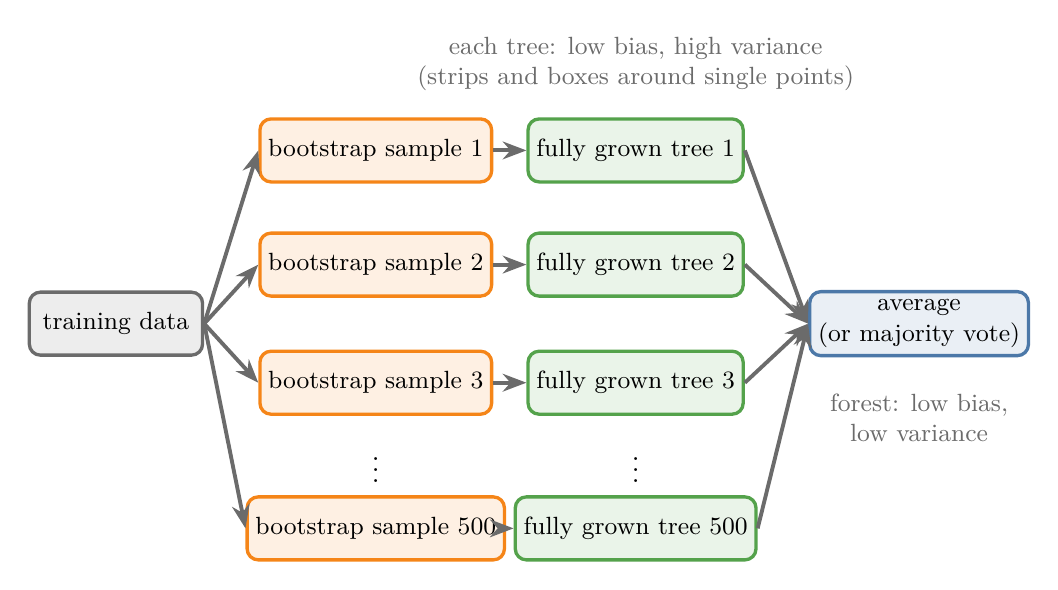
\begin{tikzpicture}[b/.style={box=#1, minimum width=2.2cm, minimum height=0.8cm, inner sep=3pt, font=\sffamily\small}]
  \node[b=cgrey] (d) at (0, 0) {training data};
  \foreach \i/\y in {1/2.2, 2/0.75, 3/-0.75} {
    \node[b=corange] (s\i) at (3.3, \y) {bootstrap sample \i};
    \node[b=cgreen, align=center] (t\i) at (6.6, \y) {fully grown tree \i};
    \draw[arrow] (d.east) -- (s\i.west); \draw[arrow] (s\i) -- (t\i);
  }
  \node at (3.3, -1.75) {$\vdots$}; \node at (6.6, -1.75) {$\vdots$};
  \node[b=corange] (s4) at (3.3, -2.6) {bootstrap sample 500};
  \node[b=cgreen] (t4) at (6.6, -2.6) {fully grown tree 500};
  \draw[arrow] (d.east) -- (s4.west); \draw[arrow] (s4) -- (t4);
  \node[b=cblue, align=center] (avg) at (10.2, 0) {average\\(or majority vote)};
  \foreach \i in {1,2,3,4} \draw[arrow] (t\i.east) -- (avg.west);
  \node[note, align=center] at (6.6, 3.3) {each tree: low bias, high variance\\(strips and boxes around single points)};
  \node[note, align=center] at (10.2, -1.2) {forest: low bias,\\low variance};
\end{tikzpicture}
\end{document}
